\begin{figure}
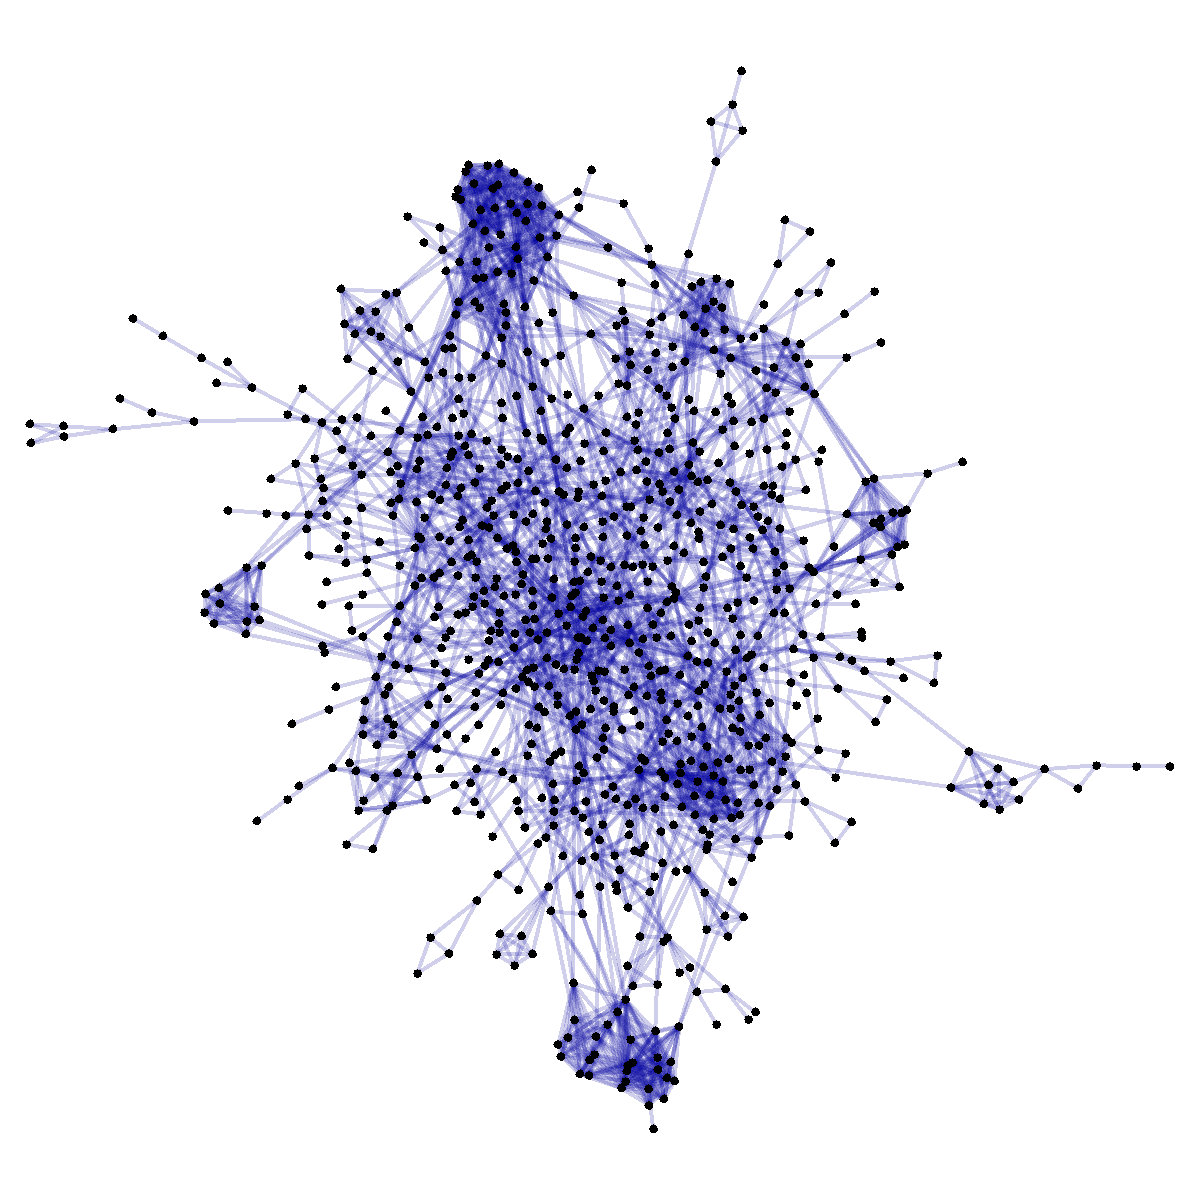
\includegraphics[height=8cm]{disconnecting_graph.png}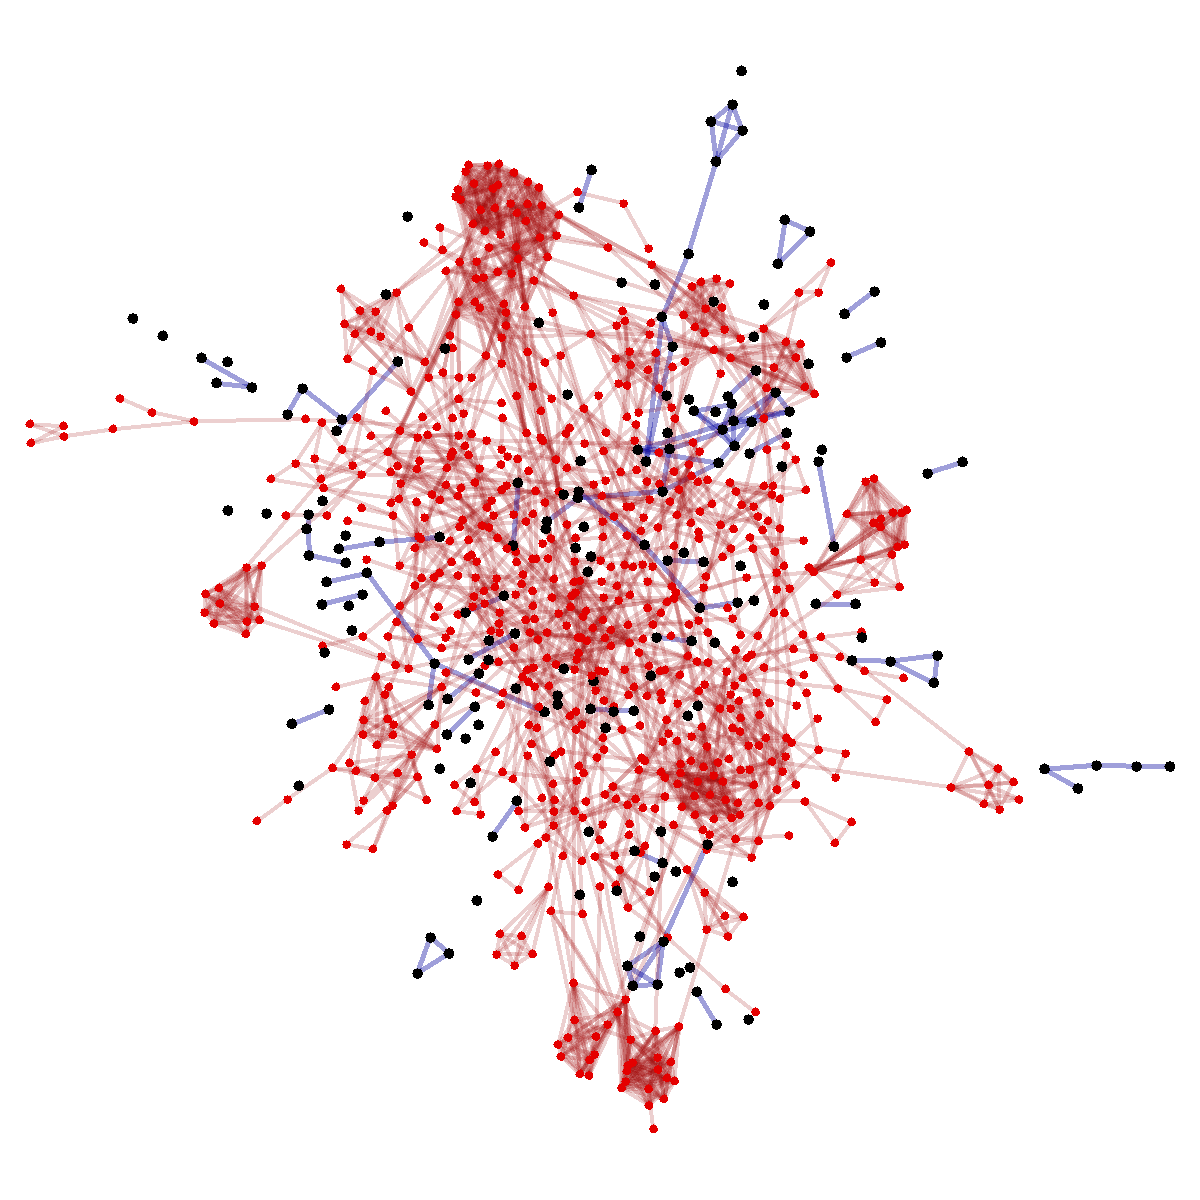
\includegraphics[height=8cm]{disconnecting_graph2.png}
\caption{Illustrated is how thresholding (a subgraph of) a protein network (left) results in one giant component (red) and multiple small disconnected components.
The left is a certain subgraph of the \textit{ecoli} dataset (all edges with confidence $>0.4$), the right graph has only edges with confidence $>0.5$.}
\label{fig:disconnecting_graph}
\end{figure}
